% Supplementary Information. Figure PDFs live in figures/ alongside the
% main-text ones; every number here is traceable to a provenance JSON in
% figures/paper/ or to the artifact named in the caption.
\clearpage
\setcounter{figure}{0}
\setcounter{table}{0}
\renewcommand{\thefigure}{S\arabic{figure}}
\renewcommand{\thetable}{S\arabic{table}}

\begin{figure}[!htbp]
 \centering
 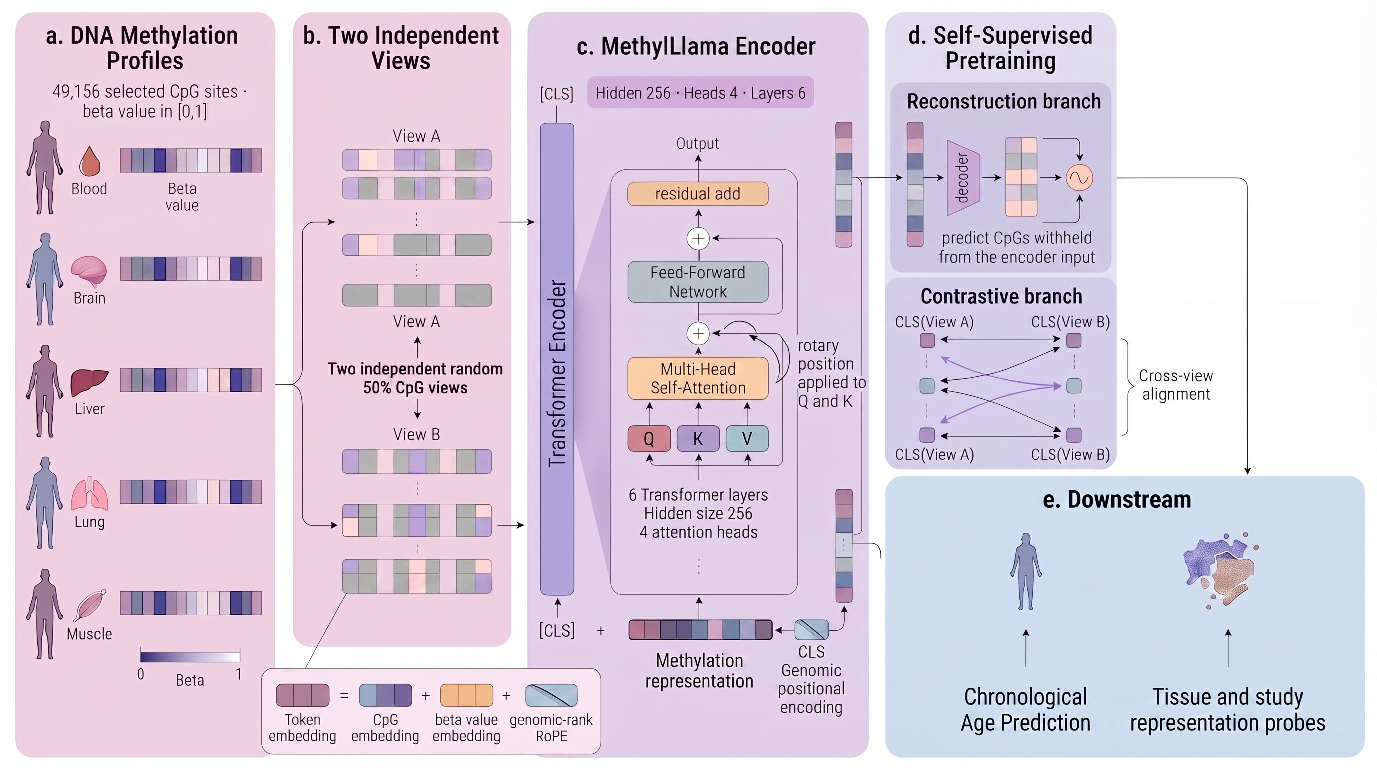
\includegraphics[width=\linewidth]{figS1_architecture.pdf}
 \caption{\textbf{\method{} architecture and the WCED pretraining objective.}
 \textbf{a}, Partial-view inputs and token construction. Two independently sampled 50\% CpG
 views are drawn from each profile. Each input token combines a learned CpG-identity embedding
 with a continuous $\beta$-value encoding; genomic position is not added to the token.
 \textbf{b}, Shared encoder. Six Transformer layers of hidden size 256 with four attention
 heads process each view alongside a prepended CLS token. Genomic rank enters exclusively as
 rotary position applied to the query and key projections inside self-attention; the value
 projection is unchanged. \textbf{c}, Dual self-supervised objectives. A shared decoder predicts
 CpGs withheld from each view using its CLS representation, while symmetric InfoNCE aligns the
 two views of one profile against other profiles in the batch. \textbf{d}, Downstream reuse of
 the pretrained encoder for chronological-age fine-tuning and frozen tissue and study probes.
 Schematic only; no measured data are plotted.}
 \label{fig:sup-architecture}
\end{figure}

\begin{figure}[!htbp]
 \centering
 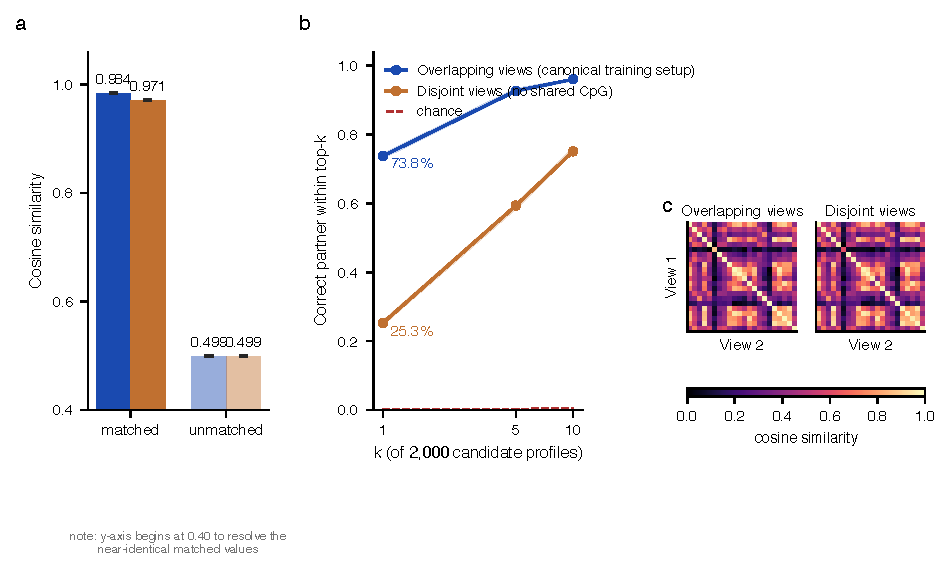
\includegraphics[width=\linewidth]{figS_view_design.pdf}
 \caption{\textbf{Cross-view consistency depends partly on overlap between the two views.}
 Two view constructions were compared on the same 2,000 profiles using the same pretrained
 encoder: the canonical training construction, in which the two 50\% CpG subsets are drawn
 independently and therefore share approximately half of their sites, and a disjoint
 construction, in which the subsets partition the valid CpGs and share none. \textbf{a}, Mean
 cosine similarity for matched and unmatched pairs. Bars show the mean and error bars the
 standard deviation across five independent random view draws. The vertical axis begins at 0.40
 so that the near-identical matched values remain distinguishable. \textbf{b}, Retrieval
 accuracy as a function of the number of candidates considered. Lines show the mean and shading
 the minimum--maximum range across the same five draws; the dashed line is chance.
 \textbf{c}, Similarity matrices for one draw under each construction (22 profiles drawn at
 random under a fixed seed, shared colour scale). Matched similarity is nearly unchanged between
 constructions (0.984 versus 0.971) whereas top-1 retrieval falls from 73.8\% to 25.3\%,
 converging again as more candidates are considered. Because the encoder was trained using
 independently sampled, potentially overlapping views, the disjoint condition is out of
 distribution for it, and these values are a conservative bound on cross-subset consistency
 rather than a matched comparison.}
 \label{fig:sup-view-design}
\end{figure}

\begin{figure}[!htbp]
 \centering
 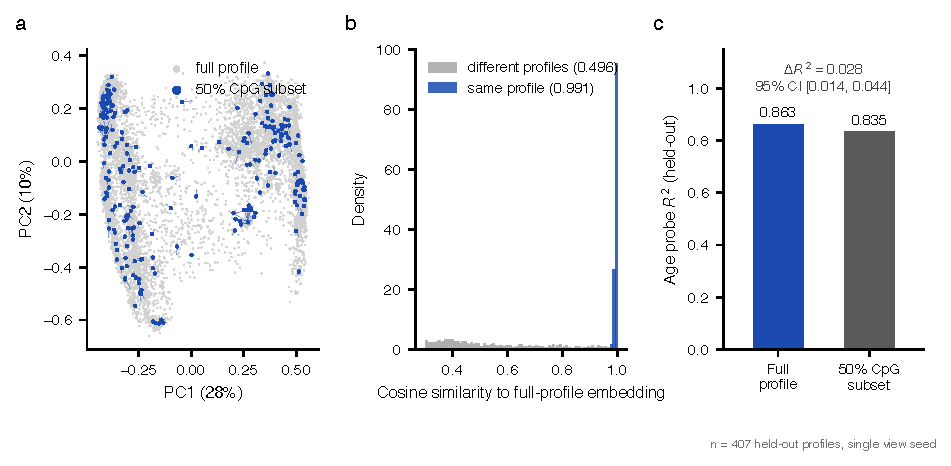
\includegraphics[width=\linewidth]{figS_panel_independence.pdf}
 \caption{\textbf{Robustness of pretrained representations to random CpG subsampling.}
 \textbf{a}, Complete profiles (grey) and 50\% CpG subsets of the same profiles (blue)
 projected into a shared principal-component space fitted on the complete profiles, with a
 segment joining each of 250 randomly chosen profiles to its own subset. \textbf{b},
 Per-profile cosine similarity between the complete-profile embedding and the embedding of a
 50\% subset of the same profile, against a shuffled-pairing control. \textbf{c}, A ridge age
 probe fitted on complete-profile embeddings of training profiles and applied, without
 adaptation, to complete and to 50\%-subset embeddings of 407 held-out profiles; the annotated
 interval is a paired bootstrap 95\% confidence interval on the difference over 5,000 resamples
 of those profiles. Subsets are random 50\% draws from a single view seed, not the probe set of
 a specific array generation, so this experiment does not establish independence from a real
 measurement platform. Performance is not identical: the probe falls from $R^2=0.863$ to
 $R^2=0.835$, a difference whose confidence interval excludes zero. The result therefore
 indicates substantial robustness to which CpGs are observed, not equivalence.}
 \label{fig:sup-panel-independence}
\end{figure}

\clearpage
\begin{table}[!htbp]
\centering
\caption{\textbf{Per-partition age-prediction metrics on the common 2,149-sample test set.}
Values were recomputed from saved sample-level predictions rather than read from training logs.
Every model was evaluated on the same test samples, so the dispersion across partitions
quantifies sensitivity to the supervised training partition and is not a population confidence
interval. The fold ensemble averages the five per-sample predictions.}
\label{tab:sup-folds}
\begin{tabular}{lrrr}
\toprule
Training partition & MedAE (years) & MAE (years) & $R^2$ \\
\midrule
Partition 0 & 3.126 & 4.439 & 0.9321 \\
Partition 1 & 3.213 & 4.458 & 0.9337 \\
Partition 2 & 3.209 & 4.570 & 0.9284 \\
Partition 3 & 3.152 & 4.541 & 0.9298 \\
Partition 4 & 3.144 & 4.455 & 0.9338 \\
\midrule
Mean $\pm$ SD & $3.169\pm0.040$ & $4.493\pm0.059$ & $0.9316\pm0.0024$ \\
Fold ensemble & 3.112 & 4.333 & 0.9365 \\
\bottomrule
\end{tabular}
\end{table}

\begin{table}[!htbp]
\centering
\caption{\textbf{Geometry of the frozen pretrained representation.}
Computed over all 10,988 profiles of the AltuMAge collection using the pretrained encoder
without fine-tuning. Effective rank is the exponential of the entropy of the normalized
singular-value spectrum; anisotropy is the mean pairwise cosine similarity, for which lower
values indicate a less directionally collapsed space. The CLS representation occupies a
substantially higher-dimensional and less anisotropic subspace than uniform pooling over
contextual CpG tokens of the same model.}
\label{tab:sup-geometry}
\begin{tabular}{lrr}
\toprule
 & CLS representation & Mean-pooled CpG tokens \\
\midrule
Effective rank & 18.12 & 3.40 \\
Mean cosine anisotropy & 0.500 & 0.867 \\
Mean $L_2$ norm & 10.01 & 5.36 \\
\bottomrule
\end{tabular}
\end{table}

\clearpage
\subsection*{Supplementary Note 1: genomic-rank rotary position encoding}

To probe the representational effect of supplying genomic rather than sequential positions to
the rotary position encoding, we trained a matched pilot pair on the same fixed 5,000-profile
subset. The two runs shared architecture, objective, and hyperparameters; the intended
difference was whether rotary position encoding received genomic-rank or sequential position
indices.

For the genomic-rank model, the mean cosine similarity of contextualized CpG representations
was 0.9831 for genomically adjacent CpGs and 0.8857 for random pairs, a locality gap of 0.0974.
Without genomic positions the corresponding values were 0.9931 and 0.9621, a gap of 0.0310. The
separation of adjacent from random CpGs was therefore approximately 3.14-fold larger with
genomic positions. In the production model's static token-embedding table, adjacent and random
CpGs showed no positive locality gap, which is consistent with locality arising through
contextual computation rather than through clustering of identity embeddings.

This is a pilot and is reported as such. It used a single seed, and the selected genomic-rank
checkpoint also had better reconstruction diagnostics than the non-genomic checkpoint
(normalized reconstruction loss 0.0906 versus 0.1585; Pearson correlation 0.9357 versus
0.9017), so the two runs are not matched on training quality and the locality difference cannot
be cleanly attributed to the position encoding alone. We make no claim that genomic-rank
positions improve downstream predictive performance; establishing that would require replicated
pretraining runs and a matched downstream ablation.
